\chapter{The Swampland: Distance, de Sitter and TCC}\label{ch:swampland}

Every chapter so far has asked what string theory \emph{contains}: a spectrum, a duality group, a
moduli space, a flux superpotential. This chapter asks the opposite question. Suppose someone hands
you a perfectly sensible-looking low-energy field theory coupled to gravity---some scalars, some
gauge fields, a potential. Which of these theories can be the low-energy limit of a consistent
theory of quantum gravity, and which cannot, no matter how the ultraviolet is filled in? The
theories that cannot are said to lie in the \emph{Swampland}; the ones that can form the
\emph{Landscape}. The criteria that separate the two are, with one or two exceptions, conjectures:
they are supported by string-theoretic examples and by general arguments about black holes and
horizons, but they are not derived from first principles \source{Pal \S1, ll.~395--430}. A student
should care for two reasons. First, the conjectures make sharp, testable statements about
cosmology---the fate of the dark energy, the maximal duration of inflation---so they are the place
where the abstract machinery of the earlier chapters touches observation. Second, the very first
example of a Swampland criterion is the circle of \cref{ch:circle,ch:tduality}: the two towers of
momentum and winding states, exchanged by T-duality, are exactly what the distance conjecture
predicts must exist at the two ends of the radius modulus. We derive this example in full,
state the distance, de~Sitter and trans-Planckian censorship conjectures, and then look
carefully at what it means to formalize a \emph{conjecture} in Lean: one does not prove it, one
encodes it as a hypothesis or a structure and proves what follows.

\section{Landscape and Swampland}\label{sec:swampland:landscape}
\index{Swampland}\index{Landscape}

String theory has a large number of vacua, each with its own low-energy effective theory. It is
tempting to conclude that anything goes at low energies. The point of the Swampland programme is
that this is false: the set of effective theories that arise from string theory---or, more
generally, from any consistent quantum gravity---is a strict subset of the set of theories that
look self-consistent on their own terms. Palti's definition, which we adopt, reads
\source{Pal \S1, ll.~395--405}:
\begin{quote}
The Swampland is the set of (apparently) consistent effective field theories that cannot be
completed into quantum gravity in the ultraviolet.
\end{quote}
``Apparently'' means that nothing is manifestly wrong with the theory as a quantum field theory;
the inconsistency appears only when one tries to complete it. The Landscape is the complement:
the effective theories that do arise from some vacuum. \Cref{fig:swampland:sets} shows the picture.

\begin{figure}[ht]
\centering
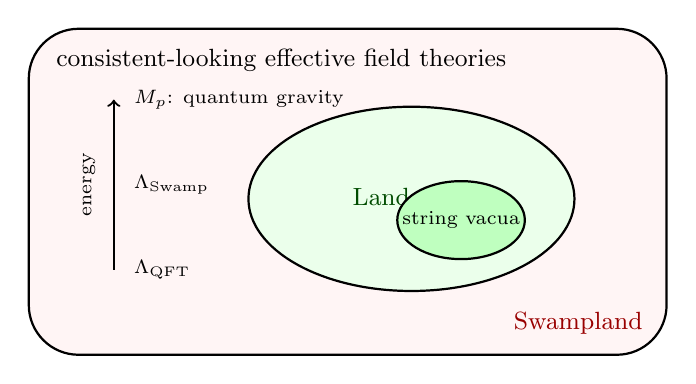
\begin{tikzpicture}[scale=0.9]
\draw[thick,rounded corners=18pt,fill=red!4] (0,0) rectangle (9,4.6);
\node[anchor=north west] at (0.25,4.45) {\small consistent-looking effective field theories};
\node[anchor=south east,text=red!60!black] at (8.8,0.15) {\small Swampland};
\draw[thick,fill=green!8] (5.4,2.2) ellipse (2.3 and 1.3);
\node[text=green!30!black] at (5.4,2.2) {\small Landscape};
\draw[thick,fill=green!25] (6.1,1.9) ellipse (0.9 and 0.55);
\node[font=\scriptsize] at (6.1,1.9) {string vacua};
\draw[->,thick] (1.2,1.2) -- (1.2,3.6);
\node[rotate=90,font=\scriptsize] at (0.85,2.4) {energy};
\node[font=\scriptsize,anchor=west] at (1.35,3.6) {$M_p$: quantum gravity};
\node[font=\scriptsize,anchor=west] at (1.35,2.4) {$\Lambda_{\rm Swamp}$};
\node[font=\scriptsize,anchor=west] at (1.35,1.2) {$\Lambda_{\rm QFT}$};
\end{tikzpicture}
\caption{Left: the scales of an effective theory coupled to gravity. Right: the Landscape of
theories that arise from quantum gravity sits inside the larger set of theories that merely look
consistent; the difference is the Swampland. After \source{Pal \S1, figs.~1, 3--4,
ll.~380--395, 492--525}.}
\label{fig:swampland:sets}
\end{figure}

A Swampland criterion has a characteristic shape \source{Pal \S1, ll.~492--525}. Take a
quantum field theory valid up to a cutoff $\Lambda_{\rm QFT}$ and couple it to gravity with a
finite Planck mass $M_p$. The conjecture is that a new scale $\Lambda_{\rm Swamp}$ appears above
which the theory must be modified---perhaps mildly, by adding a particle, perhaps drastically---if
it is ever to reach a consistent ultraviolet completion. Nothing need go wrong \emph{at}
$\Lambda_{\rm Swamp}$; rather, a theory that is not modified there is not completable. Typically
$\Lambda_{\rm Swamp}\to\infty$ as $M_p\to\infty$, since decoupling gravity removes the constraint.
The interesting regime is $\Lambda_{\rm Swamp}\ll\Lambda_{\rm QFT}\ll M_p$, where gravity
constrains physics far below the Planck scale.

Three kinds of evidence are used \source{Pal \S1, ll.~428--470}: (i)~explicit string vacua,
treated as experimental data, with the caveat that ``string-derived'' vacua (a full worldsheet
description, usually supersymmetric) and ``string-inspired'' constructions (many assumptions) carry
different weight; (ii)~general quantum-gravity arguments, mostly about black holes and
holography; (iii)~the hoped-for microscopic derivation, which does not yet exist. Because the
criteria are conjectures, every one of them is Tier~\TC{} in the language of this book, however much
evidence supports it. When a source states a conjecture we mark it \TL{} \emph{as a statement of
what the literature proposes}, never as a statement that it holds.

\begin{physicsbox}[What ``infinite distance'' will mean]
The conjectures below are phrased in terms of the moduli space of the low-energy theory, with the
metric given by the scalar kinetic terms. Moving a long way in that metric costs a lot of field
displacement in Planck units. The recurring claim is that quantum gravity does not allow such a
displacement to go unnoticed: something---an infinite tower of states---must become light, and the
effective theory must break down. The circle is the case where all of this can be computed.
\end{physicsbox}

\section{The model example: a circle}\label{sec:swampland:circle}
\index{Kaluza--Klein tower}\index{radion}

\subsection{Reduction of gravity on a circle}

Take $D=d+1$ dimensions with coordinates $X^M=(x^\mu,y)$, $\mu=0,\dots,d-1$, and let $y$ be
periodic with a \emph{fixed coordinate} period, $y\sim y+2\pi R_0$. The physical size of the circle
will be carried by a scalar field. Write the $D$-dimensional metric as
\begin{equation}\label{eq:swampland:ansatz}
\dd s_D^2 = \ee^{2a\varphi(x)}\,g_{\mu\nu}(x)\,\dd x^\mu\dd x^\nu + \ee^{2b\varphi(x)}\,\dd y^2 ,
\end{equation}
with constants $a,b$ to be fixed \source{Pal \S2.2.1, ll.~1731--1760}. The circumference measured
with the metric \eqref{eq:swampland:ansatz} is
\begin{equation}\label{eq:swampland:radius}
2\pi R = \int_0^{2\pi R_0}\sqrt{G_{yy}}\,\dd y = 2\pi R_0\,\ee^{b\varphi},
\end{equation}
so $R$ is a field, the \emph{radion}. We start from the $D$-dimensional Einstein--Hilbert action
and define the reduced Planck mass in $d$ dimensions by the coefficient of the Ricci scalar,
\begin{equation}\label{eq:swampland:eh}
S=\frac{M_D^{D-2}}{2}\int\dd^DX\sqrt{-G}\,R_D
\quad\longrightarrow\quad
S=\int\dd^dx\sqrt{-g}\Big[\frac{M_p^{d-2}}{2}R_d+\dots\Big],
\end{equation}
following \source{Pal \S1, ll.~596--612}. Two requirements fix $a$ and $b$.

\emph{The $d$-dimensional Planck mass must not depend on $\varphi$.} Otherwise the ruler with which
we measure the field distance would itself move. Splitting off the conformal factor, the metric
\eqref{eq:swampland:ansatz} is $\ee^{2a\varphi}\hat G$ with $\hat G=g\oplus\ee^{2(b-a)\varphi}\dd y^2$,
and $\sqrt{-G}=\ee^{(d+1)a\varphi}\sqrt{-\hat G}=\ee^{(d+1)a\varphi+(b-a)\varphi}\sqrt{-g}$. The Weyl
rescaling formula in $D$ dimensions, $\sqrt{-G}R_D=\sqrt{-\hat G}\,\ee^{(D-2)\omega}\big[\hat R
-2(D-1)\hat\Box\omega-(D-1)(D-2)(\hat\partial\omega)^2\big]$ with $\omega=a\varphi$, produces an
overall factor $\ee^{(d-1)a\varphi}\cdot\ee^{(b-a)\varphi}=\ee^{(b+(d-2)a)\varphi}$ in front of
$\sqrt{-g}R_d$. It is constant if and only if
\begin{equation}\label{eq:swampland:beta}
b=-(d-2)\,a .
\end{equation}
With this choice $M_p^{d-2}=M_D^{D-2}\cdot 2\pi R_0$, a constant; the $d$-dimensional metric $g$ is
the \emph{Einstein-frame} metric.\index{Einstein frame}

\emph{The radion must be canonically normalized.} Collect the $(\partial\varphi)^2$ terms. The
warped metric $\hat G$ has $\hat R=R_d-2\gamma\Box\varphi-2\gamma^2(\partial\varphi)^2$ with
$\gamma=b-a$ (the standard formula for a product with one warped flat direction), and
$\hat\Box\omega=\Box\omega+\gamma\,\partial\varphi\cdot\partial\omega$. Because the prefactor is
constant, all $\Box$ terms are total derivatives. What remains is
\[
\sqrt{-G}R_D \simeq \sqrt{-g}\big[R_d-\big(2\gamma^2+2d\gamma a+d(d-1)a^2\big)(\partial\varphi)^2\big]
= \sqrt{-g}\big[R_d-(d-1)(d-2)\,a^2\,(\partial\varphi)^2\big],
\]
where the last step uses $\gamma=-(d-1)a$ from \eqref{eq:swampland:beta}. (We checked the
algebra symbolically; it is a two-line exercise once $\gamma$ is substituted.) Multiplying by
$\tfrac12M_D^{D-2}\cdot2\pi R_0=\tfrac12M_p^{d-2}$, and setting $M_p=1$, the reduced action is
$\int\sqrt{-g}\,[\tfrac12R_d-\tfrac12(d-1)(d-2)a^2(\partial\varphi)^2]$. The kinetic term is
$-\tfrac12(\partial\varphi)^2$ precisely when
\begin{equation}\label{eq:swampland:alpha}
a^2=\frac{1}{(d-1)(d-2)},\qquad b=-\sqrt{\frac{d-2}{d-1}} .
\end{equation}
In $d=4$: $a=1/\sqrt6\approx0.408$, $b=-\sqrt{2/3}\approx-0.816$.

\begin{pitfallbox}[Two normalizations differ by $\sqrt2$]
Palti writes the reduced action as $\int\sqrt{-g}\,[R-\tfrac12(\partial\phi)^2]$ and correspondingly
finds $\alpha^2=1/(2(d-1)(d-2))$ for the metric exponent \source{Pal \S2.2.1, ll.~1755--1792}. His
field $\phi$ and ours are related by $\phi=\sqrt2\,\varphi$, since $R-\tfrac12(\partial\phi)^2
=2[\tfrac12R-\tfrac14(\partial\phi)^2]$. Every exponent quoted below in the form $\ee^{\lambda\varphi}$
becomes $\ee^{(\lambda/\sqrt2)\phi}$ in his convention. The distance conjecture only fixes an
order-one exponent, but if you compare numbers between papers you must track this factor; the
frequently quoted ``$\alpha=\sqrt3/2$'' and ``$\lambda=\sqrt{3/2}$'' for the four-dimensional circle
are the same statement.
\end{pitfallbox}

\subsection{The Kaluza--Klein tower}

Now add a massless $D$-dimensional scalar $\Psi$. Periodicity in $y$ forces a Fourier expansion
with quantized momentum along the circle,
\[
\Psi(x,y)=\sum_{n\in\Z}\psi_n(x)\,\ee^{\ii ny/R_0},\qquad -\ii\partial_y\Psi=\frac{n}{R_0}\Psi ,
\]
\source{Pal \S2.2.1, ll.~1793--1840}. The wave equation $G^{MN}\partial_M\partial_N\Psi=0$ in the
metric \eqref{eq:swampland:ansatz}, at constant $\varphi$ and with $g=\eta$, reads
\[
\ee^{-2a\varphi}\,\partial^\mu\partial_\mu\psi_n-\ee^{-2b\varphi}\frac{n^2}{R_0^2}\,\psi_n=0 ,
\]
so the Einstein-frame mass of the $n$-th mode is
\begin{equation}\label{eq:swampland:mkk}
m_n^2=\ee^{2(a-b)\varphi}\frac{n^2}{R_0^2}=\ee^{2(d-1)a\varphi}\frac{n^2}{R_0^2},
\qquad
m_n=\frac{|n|}{R_0}\,\ee^{\lambda_{\rm KK}\varphi},\quad
\lambda_{\rm KK}=(d-1)a=\sqrt{\frac{d-1}{d-2}} .
\end{equation}
Written in terms of the physical radius, $m_n\propto R^{-(d-1)/(d-2)}$: one factor $1/R$ is the
naive Kaluza--Klein mass, the extra $R^{-1/(d-2)}$ is the Einstein-frame conversion. As a check by
another route: $M_p^{d-2}=M_D^{d-1}\cdot2\pi R$ if $R$ is measured in $D$-dimensional Planck units,
so $m_n/M_p=(M_D/M_p)\,(1/RM_D)\propto(RM_D)^{-1/(d-2)-1}$, the same power. The whole tower
$\{m_n\}$ moves rigidly, with the single scale $M_{\rm KK}=\ee^{\lambda_{\rm KK}\varphi}/R_0$: as
$\varphi\to-\infty$ (large circle, since $b<0$) it becomes light \emph{exponentially in the
canonically normalized field}. This part is pure field theory.

\subsection{The winding tower and T-duality}
\index{winding tower}\index{T-duality!and the distance conjecture}

In string theory the circle carries a second tower. In the string frame the closed-string mass
formula of \cref{ch:circle} is
\begin{equation}\label{eq:swampland:stringmass}
M^2=\frac{n^2}{R^2}+\frac{w^2R^2}{\ap^2}+\frac{2}{\ap}\big(N+\tilde N-2\big),\qquad
N-\tilde N=nw ,
\end{equation}
\source{Tong \S8.1, ll.~11371--11475}, \source{Pal \S2.2.2, ll.~1854--1990}, and it is invariant
under $R\mapsto\ap/R$, $n\leftrightarrow w$. Converting to the Einstein frame requires two steps
that Palti spells out \source{Pal \S2.2.2, ll.~1974--2046}: the frame factor $\ee^{2a\varphi}$
multiplies all masses squared, and the $d$-dimensional dilaton $\Phi_d=\Phi-\tfrac12\ln(2\pi RM_s)$
is held fixed while $R$ varies, which makes the string scale $M_s\propto(2\pi R)^{1/(d-2)}$ in
$d$-dimensional Planck units. The result, in units where the coordinate period is one, is
\begin{equation}\label{eq:swampland:einsteinmass}
M_{n,w}^2=(2\pi R)^{-\frac{2}{d-2}}\Big(\frac nR\Big)^2+(2\pi R)^{\frac{2}{d-2}}\Big(\frac{wR}{\ap_0}\Big)^2 ,
\end{equation}
where $\ap_0$ is the string scale with the $R$-dependence removed. The first term reproduces the
field-theory result \eqref{eq:swampland:mkk}. The two mass scales therefore behave as
\begin{equation}\label{eq:swampland:towers}
M_{\rm KK}\propto R^{-\frac{d-1}{d-2}}\propto\ee^{+\lambda_{\rm KK}\varphi},\qquad
M_{w}\propto R^{+\frac{d-1}{d-2}}\propto\ee^{-\lambda_{\rm KK}\varphi},\qquad
M_{\rm KK}\,M_w=\text{const} ,
\end{equation}
\source{Pal \S2.2.3, ll.~2066--2100}. The product being independent of $\varphi$ is T-duality
in Einstein-frame clothing: the $\Z_2$ that exchanges the towers acts as $\varphi\mapsto-\varphi$
about the self-dual point. \Cref{fig:swampland:towers} shows the two lines.

\begin{figure}[ht]
\centering
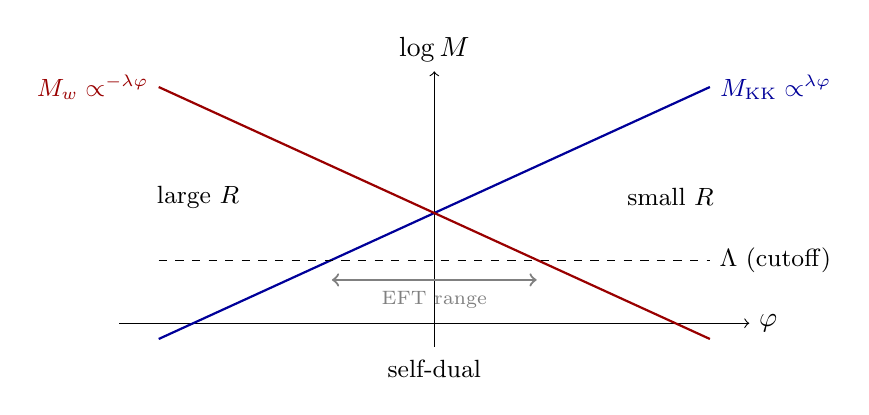
\begin{tikzpicture}[scale=1.0]
\draw[->] (-4,0) -- (4,0) node[right] {$\varphi$};
\draw[->] (0,-0.3) -- (0,3.2) node[above] {$\log M$};
\draw[thick,blue!60!black] (-3.5,-0.2) -- (3.5,3.0) node[right,font=\small] {$M_{\rm KK}\propto\ee^{\lambda\varphi}$};
\draw[thick,red!60!black] (-3.5,3.0) node[left,font=\small] {$M_w\propto\ee^{-\lambda\varphi}$} -- (3.5,-0.2);
\draw[dashed] (-3.5,0.8) -- (3.5,0.8) node[right,font=\small] {$\Lambda$ (cutoff)};
\node[font=\small,anchor=north] at (0,-0.35) {self-dual};
\node[font=\small] at (-3.0,1.6) {large $R$};
\node[font=\small] at (3.0,1.6) {small $R$};
\draw[<->,thick,gray] (-1.3,0.55) -- (1.3,0.55);
\node[font=\scriptsize,gray] at (0,0.3) {EFT range};
\end{tikzpicture}
\caption{Mass scales of the momentum and winding towers on a circle, as functions of the
canonically normalized radion $\varphi$ (Einstein frame). The slopes are $\pm\lambda_{\rm KK}$;
the $\Z_2$ symmetry of the picture is T-duality. Whichever way one moves, one tower crosses any
fixed cutoff after a finite field range. After \source{Pal \S2.2.3, fig.~8, ll.~2091--2097}.}
\label{fig:swampland:towers}
\end{figure}

\begin{example}[Numbers in four dimensions]\label{ex:swampland:numbers}
For $d=4$, $\lambda_{\rm KK}=\sqrt{3/2}\approx1.225$ in the canonical normalization. Start at the
self-dual point, where both towers have scale $M_s$, and suppose the effective theory is to be
trusted up to a cutoff $\Lambda=M_s/100$. Either tower reaches $\Lambda$ after a displacement
$|\Delta\varphi|=\ln100/\lambda_{\rm KK}\approx4.605/1.225\approx3.76\,M_p$. A displacement of
$5M_p$ towards large radius multiplies $M_{\rm KK}$ by $\ee^{-1.225\times5}\approx2.2\times10^{-3}$.
In field theory alone, moving towards \emph{small} radius would be harmless---the KK tower gets
heavier without bound. String theory forbids this: the winding tower takes over, with exactly the
same slope.
\end{example}

The observations to retain \source{Pal \S2.2.3, ll.~2113--2150} are: some tower becomes light for
either sign of $\Delta\varphi$; the behaviour is exponential in the \emph{proper} distance because
$\varphi$ is canonically normalized; the exponent is a fixed order-one number; and as
$|\Delta\varphi|\to\infty$ infinitely many states become massless, so no $d$-dimensional field theory
describes that locus---the correct description is the $D$-dimensional theory, at either end. The
lesson that string theory adds to field theory is the second tower, and it is T-duality that
supplies it.

\section{The Swampland Distance Conjecture}\label{sec:swampland:sdc}
\index{distance conjecture}\index{moduli space!metric on}\index{geodesic distance}

\subsection{Moduli space as a Riemannian manifold}

Consider a $d$-dimensional theory of gravity coupled to real scalars $\phi^i$ with no potential,
\begin{equation}\label{eq:swampland:sigma}
S=\int\dd^dx\sqrt{-g}\Big[\frac{R}{2}-\frac12\,g_{ij}(\phi)\,\partial_\mu\phi^i\partial^\mu\phi^j+\dots\Big],
\qquad M_p=1 .
\end{equation}
The scalar expectation values are coordinates on the \emph{moduli space} $\mathcal M$ and the
kinetic matrix $g_{ij}$ is a Riemannian metric on it \source{Pal \S3.6, ll.~5062--5095}. (Palti
writes the kinetic term without the $\tfrac12$; his $g_{ij}$ is half ours. Beware the clash of
notation with the spacetime metric $g_{\mu\nu}$: the two are unrelated.) The metric is positive
definite because kinetic terms have a fixed sign. The distance between two points $P,Q$ is the
length of the shortest geodesic $\gamma$ between them,
\begin{equation}\label{eq:swampland:dist}
d(P,Q)=\int_\gamma\sqrt{g_{ij}\,\frac{\dd\phi^i}{\dd s}\frac{\dd\phi^j}{\dd s}}\;\dd s .
\end{equation}
For the circle, $\mathcal M=\R$ with coordinate $\varphi$ and $g=1$, so $d(P,Q)=|\Delta\varphi|$ and
the points $\varphi=\pm\infty$ are at infinite distance from every finite point. A periodic scalar
$\phi\sim\phi+2\pi f$ with constant $f$ is the opposite case: $\mathcal M=S^1$ and no two points are
further apart than $\pi f$.

\subsection{Statement}

\begin{conjecture}[Swampland Distance Conjecture, Ooguri--Vafa; \TC]\label{conj:swampland:sdc}
Let $\mathcal M$ be the moduli space of a theory coupled to gravity, with metric from the kinetic
terms. (i)~From any point $P\in\mathcal M$ there is a point $Q\in\mathcal M$ with $d(P,Q)=\infty$.
(ii)~There is an infinite tower of states with a mass scale $M$ such that
\begin{equation}\label{eq:swampland:sdc}
M(Q)\sim M(P)\,\ee^{-\alpha\,d(P,Q)}\qquad\text{as }d(P,Q)\to\infty,
\end{equation}
for some positive constant $\alpha$. \source{Pal \S3.6, ll.~5049--5062; \S2.2.3, ll.~2167--2185}
\end{conjecture}

Three comments. First, the statement is asymptotic; the value $M(P)$ at the starting point does not
matter. Second, $\alpha$ is not specified beyond ``order one'', and the sharper reading adopted in
the literature is that the exponential behaviour sets in after a distance of one or two Planck
units. Third, the circle is the case where \eqref{eq:swampland:sdc} holds \emph{exactly}, for all
distances, with $\alpha=\lambda_{\rm KK}$; in general one must expect a bulk region of moduli space
where masses go up and down, and asymptotic regions where the exponential law takes over
\source{Pal \S3.6, ll.~5120--5150}.

The \emph{refined} version \source{Pal \S3.6, ll.~5150--5210} makes the second point quantitative and
extends the statement to fields with a potential: with $M_p$ reinstated,
\begin{equation}\label{eq:swampland:rsdc}
M(Q)<M(P)\,\ee^{-\alpha\,d(P,Q)/M_p}\qquad\text{for }d(P,Q)\gtrsim M_p,
\end{equation}
and the same holds in the field space of an effective theory even when the fields have a potential.
The inequality is now sharp, it allows faster-than-exponential decay, and it implicitly bounds
$\alpha$ from below: the tower may not grow much before the exponential decrease begins. The
tower need not consist of particles; in string examples it may be a tower of light strings,
treated as particles only below their own length scale.

\begin{physicsbox}[Why a tower, and why exponential]
Two arguments, both from \source{Pal \S3.6.1, ll.~5212--5270}. \emph{Duality.} In the circle the
two towers are exchanged by T-duality and their product is constant; moving far in either
direction makes the dual tower light. String theory has many dualities and, correspondingly, many
dual towers; the conjecture generalizes the pattern. \emph{Gravity as the weakest force.} The
scalar weak gravity conjecture asks that a particle's mass satisfy $|\partial_\phi m|>m$ for a
canonically normalized $\phi$. Maintained over a large field range this forces $m\sim\ee^{-\alpha\phi}$
with $\alpha>1$: a power law $m\sim\phi^p$ has $|\partial_\phi m|/m=p/\phi\to0$. Two particles with
oscillating masses $|\cos\phi|$, $|\sin\phi|$ can share the burden over one period, but covering a
range $2\pi N$ needs $N$ particles, and an infinite range needs an infinite tower.
\end{physicsbox}

\begin{proposition}[Exponential decay from a relative bound]\label{prop:swampland:expbound}
Let $m:[0,\infty)\to(0,\infty)$ be differentiable with $m'(\phi)\le-\alpha\,m(\phi)$ for some
$\alpha>0$ and all $\phi\ge0$. Then $m(\phi)\le m(0)\,\ee^{-\alpha\phi}$.
\end{proposition}
\begin{proof}
Set $u=\ln m$; then $u'\le-\alpha$, so $u(\phi)-u(0)=\int_0^\phi u'\le-\alpha\phi$. Exponentiate.
\end{proof}
This is the whole content of ``exponential in the distance'': a bound on the logarithmic
derivative integrates to an exponential bound. The Lean statement
\lean{sdc\_tower\_suppression} in \cref{sec:swampland:lean} is the trivial half of it, with the
exponential taken as a definition.

\subsection{What the conjecture forbids}

The first part excludes moduli spaces of finite diameter. A single periodic scalar with a
constant decay constant $f$ is therefore not allowed \emph{on its own}; it must sit inside a larger
moduli space, and in string theory the decay constant is itself a field \source{Pal \S3.6,
ll.~5110--5120}. The second part limits the validity of any effective theory with a cutoff
$\Lambda$: since the tower drops below $\Lambda$ after a finite distance, the theory is valid only in
a compact region of field space (the ``EFT range'' in \cref{fig:swampland:towers}). For inflation
this is a constraint on super-Planckian field excursions: a displacement $\Delta\phi$ costs a factor
$\ee^{-\alpha\Delta\phi}$ in the cutoff. We do not pursue the cosmological literature here; the
essential logic is \cref{ex:swampland:numbers}.

\section{The de Sitter conjecture}\label{sec:swampland:ds}
\index{de Sitter conjecture}\index{de Sitter space!entropy of}\index{quintessence}

\subsection{Statement and refinement}

A de~Sitter vacuum of string theory means a local minimum of the scalar potential at which the
potential is positive; the cosmological constant is never a free parameter but the value of $V$
at such a minimum \source{Pal \S7, ll.~10475--10500}. Constructing such minima has proved very
hard, and one may take the difficulty as a hint that they lie in the Swampland. That is not in
conflict with the observed late-time acceleration if the acceleration is driven by a slowly
rolling scalar (\emph{quintessence}) rather than by a constant \source{Pal \S7, ll.~10500--10525}.
The quantitative proposal is:

\begin{conjecture}[de Sitter conjecture, Obied--Ooguri--Spodyneiko--Vafa; \TC]\label{conj:swampland:ds}
The scalar potential of a theory coupled to gravity satisfies
\begin{equation}\label{eq:swampland:ds}
|\nabla V|\ \ge\ \frac{c}{M_p}\,V ,
\end{equation}
where $\nabla V$ is the gradient with respect to all canonically normalized scalars and $c>0$ is a
constant of order one. \source{Pal \S7, ll.~10528--10546}
\end{conjecture}

At a point with $V>0$ this forbids $\nabla V=0$: no de~Sitter minimum, and no de~Sitter maximum
either. The top of the Higgs potential is a counter-example to the bound as stated: there
$|\nabla V|/V\sim10^{-55}/M_p$ while the most negative eigenvalue of the Hessian is
$\sim-10^{35}V/M_p^2$ \source{Pal \S7, ll.~10585--10600}. The refined form accommodates it:

\begin{conjecture}[Refined de Sitter conjecture; \TC]\label{conj:swampland:rds}
Either \eqref{eq:swampland:ds} holds, or
\begin{equation}\label{eq:swampland:rds}
\min\big(\nabla_i\nabla_jV\big)\ \le\ -\frac{c'}{M_p^2}\,V ,
\end{equation}
where the left side is the smallest eigenvalue of the Hessian in an orthonormal frame and
$c'>0$ is of order one. \source{Pal \S7, ll.~10558--10585}
\end{conjecture}

The second option says: a positive plateau is allowed provided it is unstable on Hubble time
scales. The top of an axion potential of period $2\pi f$ has $\min(\nabla\nabla V)/V\le-1/f^2$, so
it satisfies \eqref{eq:swampland:rds} whenever $f\le M_p$ \source{Pal \S7, ll.~10600--10615}.

\subsection{Where the refinement comes from: entropy and the tower}

The refined conjecture was argued from the distance conjecture and the entropy of de~Sitter
space \source{Pal \S7.2, ll.~10736--10880}. We reproduce the argument because it shows how the
conjectures hang together, and because each step is an order-of-magnitude estimate that a
student should be able to reproduce.

\emph{De Sitter space in $d$ dimensions} is the hyperboloid $-X_0^2+X_1^2+\dots+X_d^2=R^2$ in
$\R^{1,d}$, with cosmological constant $\Lambda=(d-1)(d-2)/(2R^2)$; in $d=4$, $\Lambda=3/R^2$. In
static coordinates the metric $-(1-r^2/R^2)\dd t^2+(1-r^2/R^2)^{-1}\dd r^2+r^2\dd\Omega^2$ shows a
horizon at $r=R$, attached to an observer rather than to a body. It has the Gibbons--Hawking
temperature $T_{\rm dS}=1/(2\pi R)$ and, in four dimensions, the entropy
\begin{equation}\label{eq:swampland:sds}
S_{\rm dS}=8\pi^2(RM_p)^2 ,
\end{equation}
which one may try to interpret, as for black holes, as $\log\dim\mathcal H$ of a Hilbert space of
microstates \source{Pal \S7.1, ll.~10636--10700}. (The area of the horizon is $4\pi R^2$ and
$S=A/4G_N$ with $M_p^2=1/8\pi G_N$ gives $S=4\pi R^2\cdot2\pi M_p^2=8\pi^2R^2M_p^2$, consistent
with \eqref{eq:swampland:sds}.)

Now let a scalar roll on a positive potential slowly enough that the expansion accelerates. Then an
\emph{apparent} horizon exists, which requires $|\nabla V|\le\sqrt2\,V$ (if this fails the de~Sitter
conjecture already holds), and its radius is $R\sim V^{-1/2}$ from the Friedmann equation. The
covariant entropy bound assigns the entropy $\sim R^2$ to it. Meanwhile, by the distance
conjecture, the number $N$ of light tower states grows with the distance travelled,
\begin{equation}\label{eq:swampland:N}
N\sim n(\phi)\,\ee^{k\phi},
\end{equation}
with $n(\phi)$ monotonically increasing (more towers) and $k$ of order one. The entropy of the tower
is estimated as $S_{\rm tower}\sim N^\gamma R^\delta$ with unknown order-one $\gamma,\delta$. The
crucial assumption is that the tower dominates the Hilbert space, so that
\begin{equation}\label{eq:swampland:equate}
R^2\sim N^\gamma R^\delta\quad\Longrightarrow\quad
V\sim R^{-2}\sim N^{-\frac{2\gamma}{2-\delta}}\sim\ee^{-\frac{2k\gamma}{2-\delta}\phi} ,
\end{equation}
\source{Pal \S7.2, ll.~10785--10840}. Differentiating,
\begin{equation}\label{eq:swampland:c}
\frac{|\nabla V|}{V}\sim c,\qquad c\sim\frac{2k\gamma}{2-\delta} ,
\end{equation}
which is \eqref{eq:swampland:ds}. The second condition \eqref{eq:swampland:rds} marks where the
argument fails: the de~Sitter temperature gives scalars a positive mass squared of order $V$ at
horizon scales, so a tachyonic direction only destabilizes the horizon---and destroys the entropic
reading---if its magnitude exceeds $V/M_p^2$ \source{Pal \S7.2, ll.~10855--10870}.

\begin{example}[Reading off $c$]
With the simplest guesses $\gamma=1$ (entropy proportional to the number of light species) and
$\delta=0$, \eqref{eq:swampland:c} gives $c\sim k$: the steepness of the potential is the growth
rate of the tower. For the circle with $M_{\rm KK}\propto\ee^{-\lambda_{\rm KK}|\varphi|}$ towards
large radius, the number of KK states below a fixed cutoff grows as $N\sim\Lambda/M_{\rm KK}\propto
\ee^{\lambda_{\rm KK}|\varphi|}$, so $k=\lambda_{\rm KK}=\sqrt{3/2}$ in $d=4$ and the estimate is
$c\sim1.2$. This is only an illustration of the logic; the argument is valid only at
parametrically large distance, where any coupling of string theory becomes weak and a runaway
direction opens---a generalization of the Dine--Seiberg problem \source{Pal \S7.2,
ll.~10870--10880}.
\end{example}

\subsection{Cosmological consequences}

If $V>0$ today and \eqref{eq:swampland:ds} holds, the universe is not at a minimum but rolling.
A rolling scalar has equation of state
\begin{equation}\label{eq:swampland:eos}
p=\omega\rho,\qquad
\omega\simeq\frac{\tfrac12\dot\phi^2-V}{\tfrac12\dot\phi^2+V},
\end{equation}
so $\omega=-1$ is the cosmological-constant limit and dynamical dark energy has $\omega>-1$ and
time-dependent \source{Pal \S7.4, ll.~11388--11430}. Current bounds on $\omega$ translate into
$c<0.6$; the non-observation of primordial tensor modes gives $c<0.09$ in single-field slow-roll
inflation, and plateau models need $c<0.02$, in some tension with ``$c$ of order one''
\source{Pal \S7.4, ll.~11430--11465}. The conjecture thus makes the dark energy a falsifiable
statement about $\omega(t)$; it also predicts that the rolling field eventually reaches large
values where the light tower of the distance conjecture matters, with a phase transition of
unknown timing \source{Pal \S7.4, ll.~11465--11480}.

\section{Trans-Planckian censorship}\label{sec:swampland:tcc}
\index{trans-Planckian censorship conjecture}\index{TCC}\index{inflation!and TCC}

The third conjecture is not in this book's library of sources (Palti's review predates it); we
state it and derive its two standard consequences on the page. Everything in this section is
``standard; not checked against a source in this book's library''.

\begin{conjecture}[Trans-Planckian Censorship Conjecture, Bedroya--Vafa; \TC]\label{conj:swampland:tcc}
In an expanding universe that arises from a consistent theory of quantum gravity, no mode whose
physical wavelength was ever shorter than the Planck length $\ell_p=1/M_p$ can become larger than
the Hubble radius $H^{-1}$ and freeze out as a classical perturbation.
\end{conjecture}

\begin{proposition}[e-fold bound]\label{prop:swampland:efolds}
Consider expansion from time $t_i$ to $t_f$ with scale factor $a(t)$ and Hubble rate $H=\dot a/a$.
The conjecture is equivalent to
\begin{equation}\label{eq:swampland:tcc}
\frac{a_f}{a_i}<\frac{M_p}{H_f},\qquad\text{i.e.}\qquad
N\equiv\ln\frac{a_f}{a_i}<\ln\frac{M_p}{H_f},
\end{equation}
where $H_f=H(t_f)$.
\end{proposition}
\begin{proof}
A comoving mode with physical wavelength $\ell_p$ at $t_i$ has wavelength $\ell_p\,a_f/a_i$ at
$t_f$. It has crossed the Hubble radius at $t_f$ if $\ell_p\,a_f/a_i\ge H_f^{-1}$. Every mode
that was sub-Planckian at $t_i$ is shorter than this one at all later times, so forbidding the
crossing for the mode of wavelength exactly $\ell_p$ forbids it for all of them; that condition
is $a_f/a_i<H_f^{-1}/\ell_p=M_p/H_f$. Requiring it for every $t_i$ gives the conjecture.
\end{proof}

\begin{example}[Inflation at a high scale]
For $H_f=10^{13}\,$GeV and $M_p=2.4\times10^{18}\,$GeV \source{Pal \S1, ll.~606--612},
$\ln(M_p/H_f)\approx12.4$: fewer than thirteen e-folds are allowed, far short of the fifty to
sixty usually required. Conversely, sixty e-folds at constant $H$ need
$H<M_p\ee^{-60}\approx2\times10^{-8}\,$GeV.
Which of these numbers is the relevant bound depends on how many e-folds are actually needed at a
given scale, itself a function of $H$; the exercise at the end of the chapter takes this further.
\end{example}

\begin{proposition}[Asymptotic steepness from TCC]\label{prop:swampland:tccslope}
Let a canonically normalized scalar $\phi$ roll on a positive potential $V(\phi)$ in $d=4$ with
$M_p=1$, and suppose the trajectory reaches infinite distance ($\phi\to\infty$) at late times.
Then \eqref{eq:swampland:tcc} for arbitrarily late $t_f$ implies
\begin{equation}\label{eq:swampland:tccslope}
\frac{|V'|}{V}\ \ge\ \sqrt{\frac23}\qquad\text{asymptotically},
\end{equation}
and in $d$ dimensions the bound is $2/\sqrt{(d-1)(d-2)}$.
\end{proposition}
\begin{proof}
The Friedmann equation is $3H^2=\tfrac12\dot\phi^2+V$, so $\dot\phi^2\le6H^2$ and
$H/|\dot\phi|\ge1/\sqrt6$. The e-folds accumulated while $\phi$ moves from $\phi_i$ to $\phi_f$ are
$N=\int H\,\dd t=\int H\,\dd\phi/|\dot\phi|\ge(\phi_f-\phi_i)/\sqrt6$. Also $3H_f^2\ge V(\phi_f)$,
so $\ln(1/H_f)\le-\tfrac12\ln V(\phi_f)+\tfrac12\ln3$. Inserting both in \eqref{eq:swampland:tcc}:
$(\phi_f-\phi_i)/\sqrt6<-\tfrac12\ln V(\phi_f)+\text{const}$, i.e.
$V(\phi_f)<C\,\ee^{-(2/\sqrt6)\phi_f}$ for all large $\phi_f$. Hence $-\ln V(\phi)/\phi\ge
2/\sqrt6=\sqrt{2/3}$ up to a vanishing correction, so the \emph{average} logarithmic slope of $V$
over the asymptotic region is at least $\sqrt{2/3}$; if $|V'|/V$ has a limit, the limit is at
least $\sqrt{2/3}$, which is what ``asymptotically'' means in \eqref{eq:swampland:tccslope}. In
$d$ dimensions the Friedmann equation reads
$\tfrac12(d-1)(d-2)H^2=\tfrac12\dot\phi^2+V$ and the same steps give $2/\sqrt{(d-1)(d-2)}$.
\end{proof}

The number $\sqrt{2/3}\approx0.82$ is smaller than the $\sqrt2$ that separates accelerating from
decelerating exponential potentials (for $V\propto\ee^{-\lambda\phi}$ the scaling solution has
$a\propto t^{2/\lambda^2}$, accelerating if $\lambda<\sqrt2$; symbolic check), so TCC leaves a window
$\sqrt{2/3}\le\lambda<\sqrt2$ of asymptotically accelerating potentials. It also gives the de~Sitter
conjecture a definite $c$ in the asymptotic regime---unlike the entropy argument, whose $c$ depends
on the unknown $\gamma,\delta$.

\begin{physicsbox}[The dual-scale reading of TCC]
This programme's proposal (\cref{ch:dualscale,ch:cosmology}) is that the quantity
$R_{\rm eff}=R+\ap/R\ge2\sqrt{\ap}$ acts as a minimal length: no probe resolves distances below
$2\sqrt{\ap}$ because a circle of radius $R<\sqrt{\ap}$ is the same theory as one of radius
$\ap/R>\sqrt{\ap}$. If one \emph{identifies} the physical wavelength of a mode with
$R_{\rm eff}\lambda_0$ for a comoving $\lambda_0$, sub-Planckian wavelengths never occur and the
premise of TCC is never triggered. The inequality is Tier~\TA{} mathematics; the identification
is Tier~\TC{}. In particular, it says nothing about the e-fold bound
\eqref{eq:swampland:tcc}, which concerns the expansion history and not the spectrum of a circle.
\end{physicsbox}

\section{What the machine has checked}\label{sec:swampland:lean}
\index{Lean!conjecture as hypothesis}\index{vacuous theorem}

A conjecture cannot be proved in Lean, and it should not be assumed as an axiom either (the
libraries of this book use no axioms beyond the three standard ones). What one \emph{can} do is
encode the conjecture's shape---its parameters, its inequality---as a structure or as a hypothesis,
and prove what follows. This section reads six files that do this for the three conjectures of
the chapter, in decreasing order of faithfulness, and says for each what is literally proved.

\subsection{The distance conjecture over the reals}

The file \lean{StringTheoryFormalization/StringDynamics/SwamplandSafe.lean} bundles the two numbers
of \eqref{eq:swampland:sdc} with their positivity and defines the right-hand side as a function.

\begin{leancode}
structure SDCBound where
  α : ℝ          -- decay exponent (order 1)
  α_pos : 0 < α
  m₀ : ℝ         -- initial tower mass (Planck units)
  m₀_pos : 0 < m₀

noncomputable def towerMass (bound : SDCBound) (Δ : ℝ) : ℝ :=
  bound.m₀ * Real.exp (- bound.α * Δ)

theorem sdc_tower_mass_pos (bound : SDCBound) (Δ : ℝ) :
    0 < towerMass bound Δ := by ...

theorem sdc_tower_suppression (bound : SDCBound) (Δ : ℝ) (hΔ : 0 ≤ Δ) :
    towerMass bound Δ ≤ bound.m₀ := by ...
\end{leancode}

\begin{leanbox}[Plain-language reading]
\lean{SDCBound} is a pair of positive reals $(\alpha,m_0)$; no moduli space, geodesic or tower of
states is represented. \lean{towerMass} is the function $\Delta\mapsto m_0\ee^{-\alpha\Delta}$, taken
as a \emph{definition}---the exponential law is put in by hand, not derived.
\lean{sdc\_tower\_mass\_pos} says this function is positive (a positive number times an
exponential). \lean{sdc\_tower\_suppression} says $m_0\ee^{-\alpha\Delta}\le m_0$ for $\Delta\ge0$.
Proof idea: rewrite $1$ as $\exp0$, use monotonicity of $\exp$ with $-\alpha\Delta\le0$, then scale by
$m_0>0$ (\lean{nlinarith}). This is the first line of \cref{prop:swampland:expbound} with the
exponential already assumed; the substantive content of the conjecture---that a tower
\emph{must} exist and \emph{must} decay---is not stated. The file's docstring says exactly this.
\end{leanbox}

The same file contains a declaration named \lean{de\_sitter\_conjecture}:
\begin{leancode}
theorem de_sitter_conjecture (c : ℝ) (hc : 0 < c) (V : ℝ → ℝ) (gradV : ℝ → ℝ)
    (hV : ∀ φ, 0 < V φ)
    (hgrad : ∀ φ, 0 < gradV φ) :
    ∀ φ, gradV φ ≥ c * V φ → True := by ...
\end{leancode}

\begin{pitfallbox}[A theorem whose conclusion is \lean{True}]
The conclusion of \lean{de\_sitter\_conjecture} is the proposition \lean{True}, which holds
without any hypothesis; the proof is \lean{intros; trivial} and uses none of \lean{hc},
\lean{hV}, \lean{hgrad} or the bound \lean{gradV φ ≥ c * V φ}. The theorem records the
\emph{objects} a formalization of \eqref{eq:swampland:ds} would relate ($c$, $V$, $|\nabla V|$) and
asserts nothing about them. A kernel-checked statement is only as strong as its conclusion;
always read the conclusion before the name. The file's own docstring calls this a ``vacuous
placeholder'', which is the honest description. \Cref{ex:swampland:leands} asks you to replace it
with a non-vacuous consequence.
\end{pitfallbox}

\begin{physicsbox}[What a faithful formalization would need]
A statement of \cref{conj:swampland:sdc} would need: a metric space $(\mathcal M,d)$ (a Riemannian
manifold with its geodesic distance), a family of mass functions $m_k:\mathcal M\to(0,\infty)$
indexed by the tower, and the assertion
$\forall P\,\exists\,(Q_j)_{j\in\N}:\ d(P,Q_j)\to\infty\ \wedge\ \exists\alpha>0,\
\sup_km_k(Q_j)\le\sup_km_k(P)\,\ee^{-\alpha d(P,Q_j)}$ for large $j$. As a \emph{hypothesis} on a
structure this is perfectly expressible in Lean today; what cannot be done is to discharge it, since
it is a conjecture about all consistent theories of gravity. The value of the exercise is that
consequences proved from the hypothesis are then Tier~\TA{} \emph{relative to} it.
\end{physicsbox}

\subsection{Integer shadows}

\lean{StringTheoryFoundation/StringTheory/Swampland.lean} works in $\N$ and stores the
\emph{logarithm} of the suppression:
\begin{leancode}
structure DistanceConjecture where
  alpha : Nat
  moduliDistance : Nat
  logMassSuppression : Nat := alpha * moduliDistance

theorem distance_conjecture_monotonicity (alpha d1 d2 : Nat)
    (hLe : d1 ≤ d2) :
    let dc1 : DistanceConjecture := { alpha := alpha, moduliDistance := d1 }
    let dc2 : DistanceConjecture := { alpha := alpha, moduliDistance := d2 }
    dc1.logMassSuppression ≤ dc2.logMassSuppression := ...
\end{leancode}

\begin{leanbox}[Plain-language reading]
For natural numbers, $d_1\le d_2$ implies $\alpha d_1\le\alpha d_2$ (\lean{Nat.mul\_le\_mul\_left}).
The field \lean{logMassSuppression} is $\ln(m_0/m)$ in \eqref{eq:swampland:sdc} with the distance
and the exponent restricted to integers; the exponential itself never appears. An
\emph{arithmetic shadow} of the statement ``farther means lighter''. The same file has
\lean{WGCState}, the predicate \lean{satisfiesWGC} ($q^2\ge m^2$ over $\Z$) and the instance
\lean{unit\_state\_satisfies\_wgc} for $q=m=1$, decided by \lean{decide}.
\end{leanbox}

\lean{StringTheoryFoundation/StringTheory/VafaSwampland.lean} records a value of the exponent:
\begin{leancode}
structure SwamplandTower where
  spacetimeDim : Nat
  m0 : Nat
  distance : Nat
  alphaSquareNumerator : Nat := 1
  alphaSquareDenominator : Nat := spacetimeDim - 2

theorem vafa_sdc_4d_decay_rate :
    let tower : SwamplandTower := { spacetimeDim := 4, m0 := 1, distance := 0 }
    tower.alphaSquareDenominator = 2 := by ...
\end{leancode}

\begin{leanbox}[Plain-language reading]
The theorem is $4-2=2$ in $\N$, by \lean{rfl}. The docstring attaches to the default field the
value $\alpha^2=1/(d-2)$, which is a lower bound on the exponent proposed in the literature (a
sharpening of \cref{conj:swampland:sdc}; standard, not checked against a source in this book's
library) and is \emph{not} the circle's $\lambda_{\rm KK}^2=(d-1)/(d-2)$ from
\eqref{eq:swampland:mkk}: for $d=4$ the two are $1/2$ and $3/2$. Nothing in the file connects the
number to a tower. The same file's \lean{vafa\_wgc\_weak\_coupling\_cutoff\_monotone} proves
$g_1\le g_2\Rightarrow g_1M\le g_2M$ in $\N$, a shadow of the magnetic weak gravity cutoff
$\Lambda\le gM_p$, and \lean{vafa\_u1\_gauge\_consistent} checks a Boolean predicate on the pair
$(1,\mathtt{true})$.
\end{leanbox}

\subsection{A bookkeeping predicate on K3 data}

\lean{DualScaleM24Formalization/FrontierTriad/SwamplandDistance.lean} is this programme's file.
Its arithmetic is correct; its physics labels must be read with care.
\begin{leancode}
def k3_moduli_dim : Nat := 3 * 19 + 1
theorem k3_moduli_dim_eq_58 : k3_moduli_dim = 58 := by rfl
def total_k3t2_moduli_dim : Nat := k3_moduli_dim + 22
theorem total_k3t2_moduli_dim_eq_80 : total_k3t2_moduli_dim = 80 := by rfl

def max_picard_uv : Nat := 20
def min_picard_ds : Nat := 10

structure ModuliGeometry where
  picard_number : Nat
  moduli_stabilization_positive : Bool
  tau_im_positive : Bool

def isSwamplandSafe (geom : ModuliGeometry) : Bool :=
  geom.picard_number ≤ max_picard_uv &&
  geom.picard_number ≥ min_picard_ds &&
  geom.moduli_stabilization_positive &&
  geom.tau_im_positive

theorem cooper_s10_swampland_safe : isSwamplandSafe CooperS10 = true := by decide
theorem sdc_decay_coefficient_identity :
    2 * sdc_decay_alpha_squared_num = sdc_decay_alpha_squared_den := by rfl
\end{leancode}

\begin{leanbox}[Plain-language reading]
$3\cdot19+1=58$ and $58+22=80$. The numbers are right and have a source, but not the one the
docstring gives: $58$ is the dimension of the moduli space of Einstein metrics on a K3 surface,
$O(\Gamma_{3,19})\backslash O(3,19)/(O(3)\times O(19))\times\R^+$, and $80=58+22$ adds the
$b_2=22$ B-field periods to give the moduli space of the K3 sigma model
\source{Asp \S2.4 and \S3, ll.~877--905, 1636--1672}; see \cref{ch:stringsk3}. The docstring's
``22 toroidal and Wilson-line moduli of $T^2$'' is not what the arithmetic supports.
\lean{isSwamplandSafe} is a Boolean test $10\le\rho\le20$ on a record; the bound $\rho\le20$ is
the Picard-rank bound for K3 (\cref{ch:k3lattice}), the bound $\rho\ge10$ is a stipulation of the
programme with no source, and the two Boolean flags are inputs. \lean{cooper\_s10\_swampland\_safe}
evaluates the test on the record $(19,\mathtt{true},\mathtt{true})$ by \lean{decide}; it is
Tier~\TA{} as a computation and Tier~\TC{} as a statement about any surface.
\lean{sdc\_decay\_coefficient\_identity} is $2\cdot1=2$.
\end{leanbox}

\subsection{The de Sitter and TCC problem files}

\lean{Lean5Corpus/Problems/Problem6\_FluxSwampland.lean} models the flux potential $V\propto
N^2/\mathcal V^2$ of a fourfold by its numerator:
\begin{leancode}
structure FluxVacuumState where
  flux_quanta : Nat        -- N_flux in integer units
  volume : Nat             -- V in string units
  h_flux_pos : flux_quanta ≥ 1
  h_vol_pos : volume ≥ 1

def flux_potential_numerator (s : FluxVacuumState) : Nat :=
  s.flux_quanta * s.flux_quanta
def flux_gradient_numerator (s : FluxVacuumState) : Nat :=
  2 * (s.flux_quanta * s.flux_quanta)

theorem desitter_steepness_bound (s : FluxVacuumState) :
    flux_gradient_numerator s ≥ 2 * flux_potential_numerator s := by ...
theorem no_flat_desitter_vacuum (s : FluxVacuumState) :
    ¬ (flux_gradient_numerator s = 0) := by ...
\end{leancode}

\begin{leanbox}[Plain-language reading]
For $N\ge1$: $N^2>0$ (\lean{flux\_energy\_strictly\_positive}), $2N^2\ge2N^2$
(\lean{desitter\_steepness\_bound}, closed by \lean{omega}) and $2N^2\ne0$
(\lean{no\_flat\_desitter\_vacuum}); \lean{desitter\_swampland\_master\_contract} is their
conjunction. The field \lean{volume} is never used, so the ``potential'' has no volume
dependence and the ``gradient'' is a second copy of the numerator. The physics behind the file is
sound and elementary: $V=A\mathcal V^{-2}$ has $|\partial V/\partial\ln\mathcal V|=2V$, and a pure
power of the volume can have no stationary point at $V>0$. But $\ln\mathcal V$ is not a canonically
normalized field, so the coefficient $2$ is not the $c$ of \eqref{eq:swampland:ds}, and the Lean
statement is the integer identity only.
\end{leanbox}

\lean{Lean5Corpus/Problems/Problem3\_DualScaleTCC.lean} encodes the dual-scale reading of TCC from
the box at the end of \cref{sec:swampland:tcc}:
\begin{leancode}
def planck_length : Nat := 1
def effective_wavelength_num (R : Nat) (lambda_0 : Nat) : Nat :=
  (R * R + 1) * lambda_0

theorem wavelength_strictly_super_planckian
    (R : Nat) (lambda_0 : Nat) (h_R : R ≥ 1) (h_l : lambda_0 ≥ 1) :
    effective_wavelength_num R lambda_0 ≥ 2 := by ...

structure InflationParameters where
  planck_mass : Nat
  hubble_scale : Nat
  h_sub_planckian_hubble : hubble_scale < planck_mass
  h_hubble_pos : hubble_scale ≥ 1

theorem tcc_expansion_factor_positive (p : InflationParameters) :
    p.planck_mass / p.hubble_scale ≥ 1 := by ...
\end{leancode}

\begin{leanbox}[Plain-language reading]
$(R^2+1)\lambda_0\ge2$ for naturals $R,\lambda_0\ge1$; the number $R^2+1$ is the numerator of
$R+1/R$ in string units, the same inequality as \lean{self\_dual\_is\_global\_minimum} in
\cref{ch:stabilization}. \lean{sub\_planckian\_modes\_impossible} restates it as
$\neg\big((R^2+1)\lambda_0\le1\big)$. \lean{tcc\_expansion\_factor\_positive}: if $1\le H<M$ in
$\N$ then the integer quotient $M/H$ is at least $1$. \lean{tcc\_cosmic\_protection\_contract} is
the conjunction of the three. None of these mentions a scale factor, a horizon or a mode
crossing it; \eqref{eq:swampland:tcc} is not formalized. The docstring's claim that TCC is
``satisfied unconditionally'' is the Tier~\TC{} identification of the box, not a theorem.
\end{leanbox}

\begin{table}[ht]
\centering\small
\begin{tabular}{@{}p{0.41\textwidth}p{0.09\textwidth}p{0.42\textwidth}@{}}
\toprule
Statement & Tier & Evidence\\
\midrule
Reduction \eqref{eq:swampland:beta}--\eqref{eq:swampland:alpha}; KK masses
 \eqref{eq:swampland:mkk} & derived & Pal \S2.2.1; symbolic check\\
Einstein-frame towers \eqref{eq:swampland:einsteinmass}--\eqref{eq:swampland:towers},
 $M_{\rm KK}M_w$ const & \TL & Pal \S2.2.2--2.2.3; symbolic check\\
Distance conjecture, refined form & \TC & stated in Pal \S3.6\\
\Cref{prop:swampland:expbound} & derived & two lines\\
de Sitter conjecture, refined form & \TC & stated in Pal \S7\\
Entropy argument, $c\sim2k\gamma/(2-\delta)$ & \TC & Pal \S7.2; symbolic check\\
$c<0.6$ (dark energy), $c<0.09$ (tensors) & \TL & Pal \S7.4\\
TCC; e-fold bound; slope $2/\sqrt{(d-1)(d-2)}$ & \TC & standard, not in library; derived\\
$m_0\ee^{-\alpha\Delta}>0$, $\le m_0$ for $\Delta\ge0$ (over $\R$) & \TA &
 \lean{sdc\_tower\_mass\_pos}, \lean{sdc\_tower\_suppression}\\
$d_1\le d_2\Rightarrow\alpha d_1\le\alpha d_2$; $4-2=2$ ($\N$) & \TA &
 \lean{distance\_conjecture\_monotonicity}, \lean{vafa\_sdc\_4d\_decay\_rate}\\
$3\cdot19+1=58$, $58+22=80$; Boolean test on a record & \TA &
 \lean{k3\_moduli\_dim\_eq\_58}, \lean{cooper\_s10\_swampland\_safe}\\
$N^2>0$, $2N^2\ge2N^2$, $2N^2\ne0$ ($\N$) & \TA & \lean{desitter\_swampland\_master\_contract}\\
$(R^2+1)\lambda_0\ge2$; $M/H\ge1$ ($\N$) & \TA & \lean{tcc\_cosmic\_protection\_contract}\\
\lean{de\_sitter\_conjecture} & vacuous & conclusion \lean{True}\\
$R_{\rm eff}\ge2\sqrt{\ap}$ censors trans-Planckian modes & \TC & none\\
\bottomrule
\end{tabular}
\caption{Epistemic status of the statements of this chapter. All Lean theorems listed depend
only on the axioms \lean{propext}, \lean{Classical.choice} and \lean{Quot.sound}. The
identification of any Lean object with a physical system is never Tier A.}
\label{tab:swampland:tiers}
\end{table}

\begin{summarybox}
\begin{itemize}[leftmargin=*,itemsep=1pt]
\item The Swampland is the set of consistent-looking effective theories with no completion into
 quantum gravity; its criteria are conjectures supported by string vacua and by black-hole
 arguments, and they are all Tier~C.
\item On a circle, the Einstein-frame radion $\varphi$ with $2\pi R=2\pi R_0\ee^{b\varphi}$,
 $b=-\sqrt{(d-2)/(d-1)}$, is canonically normalized, and the KK tower obeys
 $m_n=(|n|/R_0)\ee^{\lambda_{\rm KK}\varphi}$ exactly, with $\lambda_{\rm KK}=\sqrt{(d-1)/(d-2)}$
 ($\sqrt{3/2}$ in $d=4$). String theory adds the winding tower with the opposite slope;
 T-duality is the $\Z_2$ of the picture and makes both ends of $\mathcal M=\R$ infinite-distance
 points with a light tower.
\item Distance conjecture: from any point there is a point at infinite geodesic distance, and a
 tower with $M\sim M_0\ee^{-\alpha d}$ becomes light there. Refined: strict inequality, onset at
 $d\sim M_p$, also for fields with a potential. It bounds the field range of any effective theory.
\item de Sitter conjecture: $|\nabla V|\ge cV/M_p$; refined: or $\min\nabla\nabla V\le-c'V/M_p^2$.
 Argued from de~Sitter entropy plus the light tower; predicts rolling dark energy with $\omega>-1$
 and is constrained to $c<0.6$ by observation.
\item TCC: $a_f/a_i<M_p/H_f$, hence fewer than $\ln(M_p/H_f)$ e-folds and, asymptotically,
 $|V'|/V\ge\sqrt{2/3}$ in four dimensions.
\item In Lean a conjecture is a structure or hypothesis, never an axiom. \lean{SDCBound} and
 \lean{towerMass} encode the form of the exponential law and the two theorems prove
 positivity and non-growth of the defined function. The other files are integer shadows or
 Boolean checks; \lean{de\_sitter\_conjecture} concludes \lean{True} and proves nothing.
\end{itemize}
\end{summarybox}

\section*{Exercises}
\addcontentsline{toc}{section}{Exercises}

\begin{exercise}[$\star$]
Derive \eqref{eq:swampland:beta} directly: write $\sqrt{-G}\,G^{\mu\nu}R_{\mu\nu}$ for the ansatz
\eqref{eq:swampland:ansatz} keeping only the terms with no derivatives of $\varphi$, integrate over
$y$, and demand that the coefficient of $\sqrt{-g}R_d$ be independent of $\varphi$.
\end{exercise}

\begin{exercise}[$\star$]
From \eqref{eq:swampland:einsteinmass} show that $M_{n,0}M_{0,w}$ is independent of $R$ and that
$M_{0,w}(R)=M_{w,0}(\ap_0/R)$ up to the constant $2\pi$ factors. Which step in the derivation
uses that the $d$-dimensional dilaton, not the $D$-dimensional one, is held fixed?
\end{exercise}

\begin{exercise}[$\star\star$]
Compute $\lambda_{\rm KK}$ for $d=5$, $6$, $10$ and $26$ and show that $\lambda_{\rm KK}\to1$ as
$d\to\infty$. Then redo the reduction on a $k$-torus with all radii equal, $y^m\sim y^m+2\pi R_0$,
and show that the KK exponent becomes $\sqrt{(d+k-2)/(k(d-2))}$; check $k=1$.
\end{exercise}

\begin{exercise}[$\star\star$]
A single axion with constant decay constant $f$ has $\mathcal M=S^1$ of circumference $2\pi f$.
Show that no tower can satisfy \eqref{eq:swampland:rsdc} on it, and that if $f$ is promoted to a
field $u$ with kinetic term $f(u)^2(\partial u)^2$ and $f(u)u\le M_p$ (the axionic weak gravity
constraint), the distance along $u$ grows at most like $M_p\ln u$
\source{Pal \S3.6.1, ll.~5212--5250}. Why is a logarithmic distance exactly what an exponential
tower needs?
\end{exercise}

\begin{exercise}[$\star\star$]
In the entropy argument, take $S_{\rm tower}\sim N$ ($\gamma=1,\delta=0$) and the circle's KK
tower with cutoff $\Lambda$ at large radius. Show $N\sim\Lambda R_0\ee^{\lambda_{\rm KK}|\varphi|}$
and derive $c\sim\lambda_{\rm KK}$. Then repeat with $\delta=1$ and comment on how sensitive $c$ is
to the unknown exponents.
\end{exercise}

\begin{exercise}[$\star\star$]
For $V=V_0\ee^{-\lambda\phi}$ in $d=4$, $M_p=1$, verify that $\phi=(2/\lambda)\ln t+\phi_0$,
$a\propto t^{p}$ solves the Friedmann and Klein--Gordon equations with $p=2/\lambda^2$ and
$V_0\ee^{-\lambda\phi_0}=(12-2\lambda^2)/\lambda^4$. For which $\lambda$ is the expansion
accelerating? Check that \eqref{eq:swampland:tcc} with $t_i$ fixed and $t_f\to\infty$ is violated
for $p>1$, and compare the resulting bound on $\lambda$ with \cref{prop:swampland:tccslope}.
\end{exercise}

\begin{exercise}[$\star\star$]
Suppose inflation at a constant Hubble rate $H$ must produce enough e-folds for the largest
observed scale, $N_{\rm req}(H)=N_0+\tfrac12\ln(H/H_0)$ with constants $N_0,H_0$ (a simple model of
the dependence of the required e-folds on the reheating scale). Combine with
\eqref{eq:swampland:tcc} to obtain an upper bound on $H$, and evaluate it for $N_0=60$,
$H_0=10^{13}\,$GeV.
\end{exercise}

\begin{exercise}[$\star\star$, Lean]\label{ex:swampland:leanmono}
Using \lean{SDCBound} and \lean{towerMass}, state and prove monotonicity:
$\lean{towerMass}\ \lean{bound}\ \Delta'\le\lean{towerMass}\ \lean{bound}\ \Delta$ whenever
$\Delta\le\Delta'$. Useful lemmas: \lean{Real.exp\_le\_exp} for the exponential and
\lean{mul\_le\_mul\_of\_nonneg\_left} for the prefactor, whose non-negativity comes from the field
\lean{m₀\_pos}. Explain why \lean{sdc\_tower\_suppression} is the special case $\Delta=0$.
\end{exercise}

\begin{exercise}[$\star\star$, Lean]\label{ex:swampland:leands}
Replace the conclusion \lean{True} of \lean{de\_sitter\_conjecture} by something that uses the
hypotheses: prove that under \lean{hgrad φ ≥ c * V φ} and \lean{0 < c} one has
\lean{V φ ≤ gradV φ / c} (use \lean{le\_div\_iff₀} or \lean{div\_le\_iff₀} from Mathlib, or
\lean{nlinarith}). Then state, without proving, the real de~Sitter conjecture for a single field
as a \lean{def} of type \lean{Prop} with $V:\R\to\R$ and \lean{deriv V}.
\end{exercise}

\begin{exercise}[$\star\star\star$]
Prove the converse direction of \cref{prop:swampland:expbound} in the following form: if
$m(\phi)\le m(0)\ee^{-\alpha\phi}$ for all $\phi\ge0$ and $m$ is positive and smooth, then
$\liminf_{\phi\to\infty}(-m'/m)\ge\alpha$ need \emph{not} hold pointwise (construct a
counter-example with oscillations), but its running average
$\frac1\phi\int_0^\phi(-m'/m)$ has $\liminf\ge\alpha$. Relate this to the difference between the
original and refined distance conjectures.
\end{exercise}

\section*{Further reading}
\addcontentsline{toc}{section}{Further reading}
\begin{itemize}[leftmargin=*,itemsep=1pt]
\item Definition of the Swampland, the scale $\Lambda_{\rm Swamp}$ and the three kinds of
 evidence: \source{Pal \S1, ll.~368--530}. Conventions: \source{Pal \S1, ll.~580--612}.
\item The circle, in both frames, and the first statement of the distance conjecture:
 \source{Pal \S2.2, ll.~1716--2200}; the string-frame mass formula \source{Tong \S8.1,
 ll.~11371--11475}.
\item Distance conjecture, refined form, relation to the weak gravity conjecture and to spatial
 field variations: \source{Pal \S3.6, ll.~5049--5340}.
\item de Sitter conjecture, refinement, de~Sitter entropy, the entropy argument and the
 cosmological bounds: \source{Pal \S7, ll.~10475--10880}; \source{Pal \S7.4, ll.~11388--11480}.
\item Moduli of K3 and of the K3 sigma model, for the numbers 58 and 80:
 \source{Asp \S2.4, ll.~877--905}; \source{Asp \S3, ll.~1636--1672}.
\item Lean sources, each with a docstring that states what is and is not proved:
 \begin{itemize}[leftmargin=*,itemsep=0pt]
 \item \lean{StringTheoryFormalization/StringDynamics/SwamplandSafe.lean}
 \item \lean{StringTheoryFoundation/StringTheory/Swampland.lean}
 \item \lean{StringTheoryFoundation/StringTheory/VafaSwampland.lean}
 \item \lean{DualScaleM24Formalization/FrontierTriad/SwamplandDistance.lean}
 \item \lean{Lean5Corpus/Problems/Problem6\_FluxSwampland.lean}
 \item \lean{Lean5Corpus/Problems/Problem3\_DualScaleTCC.lean}
 \end{itemize}
\end{itemize}
